\subsection{\RU{Пример CPUID}\EN{CPUID example}}

\RU{Язык \CCpp позволяет указывать, сколько именно бит отвести для каждого поля структуры. 
Это удобно если нужно экономить место в памяти. К примеру, для переменной типа \Tbool достаточно одного бита.
Но, это не очень удобно, если нужна скорость.}
\EN{\CCpp language allow to define exact number of bits for each structure fields.
It is very useful if one needs to save memory space. 
For example, one bit is enough for variable of \Tbool type.
But of course, it is not rational if speed is important.}

\newcommand{\FNCPUID}{\footnote{\url{http://en.wikipedia.org/wiki/CPUID}}}

\index{x86!\Instructions!CPUID}
\label{cpuid}
\RU{Рассмотрим пример с инструкцией \CPUID\FNCPUID. 
Эта инструкция возвращает информацию о том, какой процессор имеется в наличии и какие возможности он имеет.}
\EN{Let's consider \CPUID\FNCPUID instruction example.
This instruction returning information about current CPU and its features.}

\RU{Если перед исполнением инструкции в \EAX будет 1, 
то \CPUID вернет упакованную в \EAX такую информацию о процессоре:}
\EN{If the \EAX is set to 1 before instruction execution, 
\CPUID will return this information packed into the \EAX register:}

\begin{center}
\begin{tabular}{ | l | l | }
\hline
3:0 (4 \bitsENRU)& Stepping \\
7:4 (4 \bitsENRU) & Model \\
11:8 (4 \bitsENRU) & Family \\
13:12 (2 \bitsENRU) & Processor Type \\
19:16 (4 \bitsENRU) & Extended Model \\
27:20 (8 \bitsENRU) & Extended Family \\
\hline
\end{tabular}
\end{center}

\newcommand{\FNGCCAS}{\footnote{\href{http://www.ibiblio.org/gferg/ldp/GCC-Inline-Assembly-HOWTO.html}
{\RU{Подробнее о встроенном ассемблере GCC}\EN{More about internal GCC assembler}}}}

\RU{MSVC 2010 имеет макрос для \CPUID, а GCC 4.4.1 ~--- нет. 
Поэтому для GCC сделаем эту функцию сами, используя его встроенный ассемблер\FNGCCAS.}
\EN{MSVC 2010 has \CPUID macro, but GCC 4.4.1~---has not.
So let's make this function by yourself for GCC with the help of its built-in assembler\FNGCCAS.}

\lstinputlisting{patterns/15_structs/6_bitfields/cpuid/CPUID.c}

\RU{После того как \CPUID заполнит \EAX/\EBX/\ECX/\EDX, у нас они отразятся в массиве \TT{b[]}. 
Затем, мы имеем указатель на структуру \TT{CPUID\_1\_EAX}, и мы указываем его на значение 
\EAX из массива \TT{b[]}.}
\EN{After \CPUID will fill \EAX/\EBX/\ECX/\EDX, these registers will be reflected in the \TT{b[]} array.
Then, we have a pointer to the \TT{CPUID\_1\_EAX} structure and we point it to the value in the \EAX from \TT{b[]} array.}

\RU{Иными словами, мы трактуем 32-битный \Tint как структуру.}
\EN{In other words, we treat 32-bit \Tint value as a structure.}

\RU{Затем мы читаем из структуры.}\EN{Then we read from the stucture.}

\subsubsection{MSVC}

\RU{Компилируем в MSVC 2008 с опцией \Ox}\EN{Let's compile it in MSVC 2008 with \Ox option}:

\lstinputlisting[caption=\Optimizing MSVC 2008]{patterns/15_structs/6_bitfields/cpuid/CPUID_msvc_Ox.asm}

\index{x86!\Instructions!SHR}
\RU{Инструкция \TT{SHR} сдвигает значение из \EAX на то количество бит, 
которое нужно \IT{пропустить}, то есть, мы игнорируем некоторые биты \IT{справа}.}
\EN{\TT{SHR} instruction shifting value in the \EAX register by number of bits must be
\IT{skipped}, e.g., we ignore a bits \IT{at right}.}

\index{x86!\Instructions!AND}
\RU{А инструкция \ANDIns очищает биты \IT{слева} которые нам не нужны, или же, говоря иначе, 
она оставляет по маске только те биты в \EAX, которые нам сейчас нужны.}
\EN{\ANDIns instruction clears bits not needed \IT{at left}, or, in other words, 
leaves only those bits in the \EAX register we need now.}

\subsubsection{MSVC + \olly}
\index{\olly}

\RU{Загрузим пример в}\EN{Let's load our example into} \olly 
\RU{и увидим, какие значения были установлены в EAX/EBX/ECX/EDX после
исполнения}\EN{and see, which values was set in EAX/EBX/ECX/EDX after execution of} CPUID: 
\figref{fig:cpuid_olly_1}.

\RU{В EAX установлено}\EN{EAX has} \TT{0x000206A7} 
(\RU{мой}\EN{my} \ac{CPU} \EN{is}\RU{---} Intel Xeon E3-1220).\\
\RU{В двоичном виде это}\EN{This is} $0000 0000 0000 0010 0000 0110 1010 0111$\EN{ in binary form}.

\RU{Вот как распределяются биты по полям в моем случае}\EN{Here is how bits are distributed by fields}:

\begin{center}
\begin{tabular}{ | l | l | l | }
\hline
\headercolor{} \RU{поле}\EN{field} &
\headercolor{} \RU{в двоичном виде}\EN{in binary form} &
\headercolor{} \RU{в десятичном виде}\EN{in decimal form} \\
\hline
reserved2		& 0000 & 0 \\
\hline
extended\_family\_id	& 00000000 & 0 \\
\hline
extended\_model\_id	& 0010 & 2 \\
\hline
reserved1		& 00 & 0 \\
\hline
processor\_id		& 00 & 0 \\
\hline
family\_id		& 0110 & 6 \\
\hline
model			& 1010 & 10 \\
\hline
stepping		& 0111 & 7 \\
\hline
\end{tabular}
\end{center}

\begin{figure}[H]
\centering
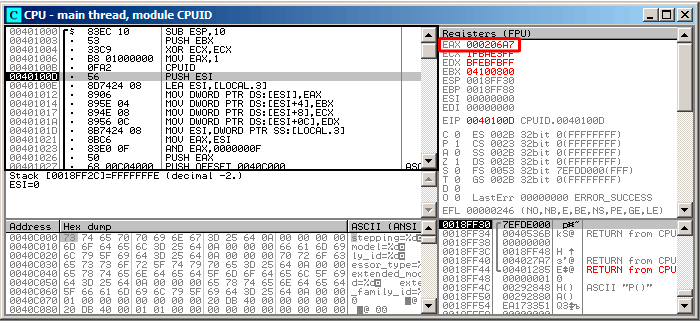
\includegraphics[scale=\FigScale]{patterns/15_structs/6_bitfields/cpuid/olly.png}
\caption{\olly: \RU{После исполнения CPUID}\EN{After CPUID execution}}
\label{fig:cpuid_olly_1}
\end{figure}

\begin{figure}[H]
\centering
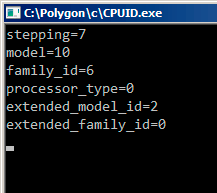
\includegraphics[scale=0.66]{patterns/15_structs/6_bitfields/cpuid/result.png}
\caption{\olly: \RU{Результат работы}\EN{Result}}
\label{fig:cpuid_olly_2}
\end{figure}

\subsubsection{GCC}

\RU{Попробуем GCC 4.4.1 с опцией \Othree.}\EN{Let's try GCC 4.4.1 with \Othree option.}

\lstinputlisting[caption=\Optimizing GCC 4.4.1]{patterns/15_structs/6_bitfields/cpuid/CPUID_gcc_O3.asm}

\RU{Практически, то же самое. Единственное что стоит отметить это то, что GCC решил зачем-то объединить 
вычисление \TT{extended\_model\_id} и \TT{extended\_family\_id} в один блок, 
вместо того чтобы вычислять их перед соответствующим вызовом \printf.}
\EN{Almost the same.
The only thing worth noting is the GCC somehow united calculation of
\TT{extended\_model\_id} and \TT{extended\_family\_id} into one block,
instead of calculating them separately, before corresponding each \printf call.}
